\chapter{Modeling}
\label{chap:modeling}

This chapter delves into the mathematical modeling of light-\gls{uvms}s. Starting with the foundational 
principles of rigid body dynamics, the chapter expands into the kinematic and 
dynamic modeling of \gls{aiauv}s, highlighting the coupling 
effects between manipulator arms and the vehicle's base. Hydrodynamic forces, 
including added mass and damping effects, are addressed to ensure an accurate 
representation of underwater motion. These mathematical models are the building
blocks for developing advanced control algorithms discussed in later chapters.

\section{Rigid Body Kinetics}

Before modeling a general \gls{uvms} with multiple links, we will model
a rigid body under water. As it turns out, the equations describing the motion
of a system with multiple links is very much related to the dynamic properties
of each individual link. This will become apparent when describing the mass
and Coriolis matrices, as well as the forces acting on the general system.
Consider a rigid body with mass $m$. Denote by $\bm{v}_{ng}^b$ the body's translational
velocity, and by $\bm{\omega}_{ng}^b$ its angular velocity in the
body-fixed frame. We can find the kinetic energy of the body by integrating the
kinetic energy of every infinitesimal mass element. The kinetic energy
of whole body is then given by
\begin{equation}
    T = \frac{1}{2} \int \bm{v}_m^T \bm{v}_m\, dm,
\end{equation}
where $\bm{v}_m$ is the velocity of the mass element.
The velocity of the mass element $\bm{v}_m$ can be expressed as
\begin{align}
    \bm{v}_m &= \bm{v}_{ng}^b + \bm{\omega}_{ng}^b \times \bm{r}_m,
\end{align}
where $\bm{r}_m$ is the position of the mass element relative to the center of
mass. By defining $\bm{\nu} = \bm{\nu}_{bg}^b = \begin{bmatrix}(\bm{v}_{ng}^b)^T & (\bm{\omega}_{ng}^b)^T \end{bmatrix}^T$, the kinetic energy can be written as
\begin{align}
    T = \frac{1}{2} \bm{\nu}^T
    \begin{bmatrix}
        \I_{3\times 3} \int \,dm & - \int [\bm{r}_m]_\times \,dm \\
        - \int [\bm{r}_m]_\times \,dm & -\int [\bm{r}_m]_\times [\bm{r}_m]_\times \,dm
    \end{bmatrix}
    \bm{\nu}\label{eq:T_body}.
\end{align}
Since the twist is defined in the center of gravity, we have that
\begin{align}
    \int [\bm{r}_m]_{\times} \,dm &= \bm{0},
\end{align}
by definition of the center of mass. The bottom right block in \autoref{eq:T_body} is recognized as the
definition of the inertia matrix $\bm{I_g^b} \in \R^{3\times 3}$. The kinetic energy can then be
expressed as
\begin{align}
    T(\bm{\nu}) &= \frac{1}{2} \bm{\nu}^T \bm{M} \bm{\nu} \label{eq:TM_body} &
    \bm{M} &= \begin{bmatrix} m\I_{3} & \bm{0} \\ \bm{0} & \bm{I}_g^b \end{bmatrix}.
\end{align}
The matrix $\bm{M}$ in \autoref{eq:TM_body} is called the spatial inertia matrix of the rigid body.
Using Lagrange's method, being careful when differentiating in a rotating frame,
we can find the equations of motion for the rigid body as \cite{fossen2021}:
\begin{align}
    \underbrace{
    \begin{bmatrix}
        m \I_{3} & \bm{0} \\
        \bm{0} & \bm{I}_g^b
    \end{bmatrix}
}_{\bm{M}_{RB}^{CG}} \dot{\bm{\nu}}
    +
    \underbrace{
    \begin{bmatrix}
        m [\bm{\omega}_{nb}^b]_{\times} & \bm{0} \\
        \bm{0} & -[\bm{I}_g^b \bm{\omega}_{nb}^b]_{\times}
    \end{bmatrix}
}_{\bm{C}_{RB}^{CG}}\bm{\nu} = \bm{\tau}
    \label{eq:rigid_body_eom_cg}
\end{align}
where $\bm{\tau}$ is the generalized forces and moments acting on the body. We call the matrices
pre-multiplying $\dot{\bm{\nu}}$ and $\bm{\nu}$ for $\bm{M}_{RB}^{CG}$ and $\bm{C}_{RB}^{CG}$ respectively. In general one might want to consider the equations of motion
about a different point than the center of gravity. The twist of the body is
related to the twist in the new point, $b$, by the matrix \cite{fossen2021}
\begin{align}
        \bm{\nu}_{ng}^{b} =
    \underbrace{
        \begin{bmatrix}
            \I_{3} & -[\bm{r}_{ng}^{b}]_{\times} \\
            \bm{0} & \I_{3}
        \end{bmatrix}
    }_{\bm{H}(\bm{r}_{ng}^b)}
    \bm{\nu}_{nb}^{b},
    \label{eq:fossen_H}
\end{align}
where $\bm{r}_{ng}^{b}$ is the position of the center of gravity relative to the
new point and $\bm{\nu}_{nb}^{b}$ is the twist in the new point. By
pre-multiplying \autoref{eq:rigid_body_eom_cg} by the inverse of the matrix
in \autoref{eq:fossen_H} we get the equations of motion about the new point:
\begin{align}
    \underbrace{
        \bm{H}^T(\bm{r}_{bg}^b) \bm{M}_{CG}^{RB} \bm{H}(\bm{r}_{bg}^b)
    }_{\bm{M}_{RB}}
    \dot{\bm{\nu}}_{nb}^b
    + \underbrace{
        \bm{H}^T(\bm{r}_{bg}^b) \bm{C}_{CG}^{RB} \bm{H}(\bm{r}_{bg}^b)
    }_{\bm{C}_{RB}}
    \bm{\nu}_{nb}^b
    = \underbrace{
        \bm{H}^T(\bm{r}_{bg}^b)
    \bm{\tau}
    }_{\bm{\tau}_{b}^b}.
\end{align}
$\bm{\tau}_{b}^b$ is the generalized forces acting on the body about the new
point. The $\bm{M}_{RB}$ and $\bm{C}_{RB}$ matrices are given by \cite{fossen2021}:
\begin{subequations}
\begin{align}
    \bm{M}_{RB} &= \begin{bmatrix}
        m \I_3 & - m [\bm{r}_{bg}^b]_{\times} \\
        m [\bm{r}_{bg}^b]_{\times} & \bm{I}_g^b - m [\bm{r}_{bg}^b]_{\times}[\bm{r}_{bg}^b]_{\times}
    \end{bmatrix} \\
    \bm{C}_{RB} &= \begin{bmatrix}
        m [\bm{\omega}_{nb}^b] & -m [\bm{\omega}_{nb}^b]_{\times}[\bm{r}_{bg}^b]_{\times} \\
        m [\bm{\omega}_{nb}^b]_{\times}[\bm{r}_{bg}^b]_{\times} & 
        -m \cross{\bm{r}_{bg}^b} \cross{\bm{\omega}_{bg}^b} \cross{\bm{r}_{bg}^b} -
        \cross{\bm{I}_g^b \bm{\omega}_{bg}^b}
    \end{bmatrix}. \label{eq:crb}
\end{align}
\end{subequations}
It can be shown that the Coriolis matrix in \autoref{eq:crb} ca be equivalently
written as \cite{sagatun1991}:
\begin{align}
    \bm{C}_{RB}(\bm\nu) = \begin{bmatrix}
        \bm{0}_{3 \times 3} & 
        -\left[\bm{M}_{11}\bm{v}_{nb}^{b} + \bm{M}_{12}\bm{\omega}_{nb}^b \right]_{\times} \\
        -\left[\bm{M}_{11}\bm{v}_{nb}^{b} + \bm{M}_{12}\bm{\omega}_{nb}^b \right]_{\times} &
        -\left[\bm{M}_{21}\bm{v}_{nb}^{b} + \bm{M}_{22}\bm{\omega}_{nb}^b \right]_{\times}
    \end{bmatrix},
\end{align}
Where $\bm{M}_{ij}$ are the $3 \times 3$ submatrices of the $\bm{M}_{RB}$ matrix.

% -----------------------------------------------------------------------------
\newpage
\section{AIAUV Modeling}

A comprehensive description of the kinematics and dynamics of
\gls{aiauv}'s can be found in \cite{schmidt2018}. Much of this section
will be based on the work of \cite{from2014} and \cite{schmidt2018}, as well as an unpublished
first draft of \cite{schmidt2018}. The following chapter will use notation adopted from
\cite{from2014}.

% -----------------------------------------------------------------------------
\subsection{Differential Kinematics}
\label{sec:diff_kin}


Consider a system with $n$ rigid links connected together with $n-1$ joints. The
links are indexed from $1$ to $n$, where the base
has index $1$ and the head has index $n$.
%The base link with index $1$ can also be referred to as the head.
\begin{figure}[h!]
    \centering
    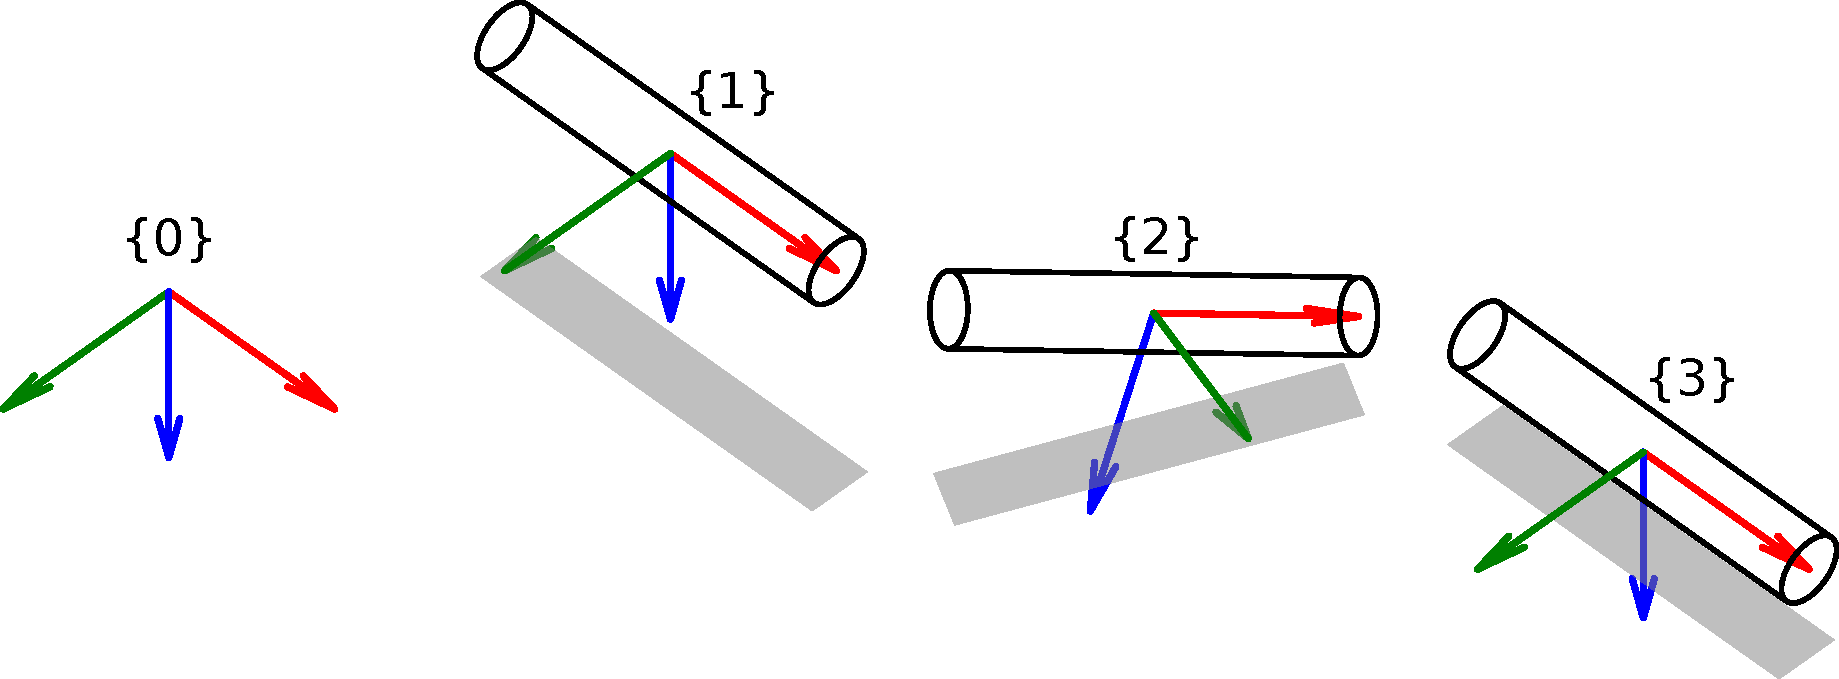
\includegraphics[width=\textwidth]{assets/frames_thin.pdf}
    \caption{Frames attached to the links of a snake-like robot.}
    \label{fig:frames}
\end{figure}
We denote some inertial \gls{ned} frame by $\{0\}$, and associate a frame to each link,
setting the frame number the same as the link number.
\autoref{fig:frames} shows an example of such a setup. Here, the system has
three links connected by two joints. To highlight the importance of the $\{0\}$-
and $\{n\}$-frames, they will also be reffered to as the $\{n\}$, for \gls{ned}, and
$\{b\}$, for body, respectively. The numbering and lettering will be used interchangeably
depending on the context.

A common way to describe the configuration of the base link is by the \gls{ned}
position and a set of Euler angles. Alterneatively, the rotation of the base link
can be described by a unit quaternion. It will be assumed that the transformations
between links are functions of a vector of joint angles, where we define
$n_j \in \mathbb{N}$ to be the total number of joint angles. Putting this together,
the necessary variables to describe the configuration of the entire system are
collected in the vector $\bm{\xi}_{\Theta} \in \R^{6+n_j}$:
%we define the configuration of the entire system as $\bm{\xi} \in \R^{6+n_j}$:
\begin{align}
    \bm{\xi}_{\Theta} &= \begin{bmatrix}\bm{\eta}_{\Theta} \\ \bm{\theta} \end{bmatrix} &
        \bm{\eta}_{\Theta} &= \begin{bmatrix}\bm{p}_{nb}^n \\ \bm{\Theta}_{nb} \end{bmatrix} &
            \bm{p}_{nb}^n &= \begin{bmatrix}x^n \\ y^n \\ z^n \end{bmatrix} &
                \bm{\Theta}_{nb} &= \begin{bmatrix}\phi \\ \theta \\ \psi \end{bmatrix} &
                    \bm{\theta} &= \begin{bmatrix}\bm{\theta}_1 \\ \vdots \\ \bm{\theta}_{n-1}\end{bmatrix},
\end{align}
where $\bm{\eta} \in \R^6$ is a collection of the the NED position $\bm{p}_{nb}^n \in \R^3$,
and Euler angles $\bm{\Theta}_{nb} \in \R^3$, of the base
link. $\bm{\theta} \in \R^{n_j}$ is the vector of joint angles, and $\bm{\theta}_i$, $i = 1,\cdots,n-1$
is a vector of joint angles for link $i$. We note that each joint can be a function of $1$ or
more joint angles.
%In the case of a unit quaternion representation of the base link,
%rotation, the vector $\bm{\Theta}_{nb}$ is replaced by a unit quaternion $\bm{q}_b^n$.
The rotation of the base link can alternatively be represented using a unit quaternion,
in that case the vector of Euler angles $\bm{\Theta}_{nb}$ is replaces by the quaternion
$\bm{q}_b^n$.
The configuration of the system is then uniquely defined by the vector $\bm{\xi}_q \in \R^{7+n_j}$.
\begin{align}
    \bm{\xi}_q &= \begin{bmatrix}\bm{\eta}_q \\ \bm{\theta} \end{bmatrix} &
        \bm{\eta}_q &= \begin{bmatrix}\bm{p}_{nb}^n \\ \bm{q}_b^n \end{bmatrix} &
            \bm{q}_{b}^n &= \begin{bmatrix}\eta \\ \bm{\epsilon} \end{bmatrix} &
                \bm{\epsilon} &= \begin{bmatrix}\epsilon_1 \\ \epsilon_2 \\ \epsilon_3 \end{bmatrix},
\end{align}
where $\eta$ is the scalar part of the quaternion and $\bm{\epsilon} \in \R^3$ is the vector part.
The quaternion satisfies the constraint $||\bm{q}_b^n||_2 = 1$. The homogeneous
transformation matrix from the base link to the inertial frame can be expressed as
\begin{align}
    \bm{H}_1^0(\bm{\eta}_{\Theta}) &= \begin{bmatrix}
        \bm{R}_b^n(\bm{\Theta})& \bm{p}_{nb}^n \\
        \bm{0}_{1\times3} & 1
    \end{bmatrix} &
    \bm{H}_1^0(\bm{\eta}_{q}) &= \begin{bmatrix}
        \bm{R}_b^n(\bm{q}_{b}^n)& \bm{p}_{nb}^n \\
        \bm{0}_{1\times3} & 1
    \end{bmatrix},
    \label{eq:H1}
\end{align}
using Euler angles and unit quaternion, respectively. In the case of Euler angles,
$\bm{R}_b^n$ uses the $x$-, $y$- and $z$-axis rotation matrices:
\begin{align}
    \bm{R}_b^n(\bm{\Theta}_{nb}) &= \bm{R}_z(\psi) \bm{R}_y(\theta) \bm{R}_x(\phi),
\end{align}
as defined in \autoref{eq:bp:so3:rotations}. Explicitly, the rotation matrix $\bm{R}_b^n$
is given by
\begin{subequations}
\begin{align}
    \bm{R}_b^n(\bm{\Theta}) &= \begin{bmatrix}
        c\psi\, c\theta & -s\psi\, c\phi + c\psi\, s\theta\, s\phi & s\psi\, s\phi + c\psi\, c\phi\, s\theta \\
        s\psi\, c\theta & c\psi\, c\phi + s\psi\, s\theta\, s\phi & -c\psi\,s\phi + s\psi\, c\phi\, s\theta \\
        -s\theta & c\theta\, s\phi & c\theta\, c\phi
    \end{bmatrix} \\
    \bm{R}_b^n(\bm{q}_b^n) &= \begin{bmatrix}
        1 - 2(\epsilon_2^2 + \epsilon_3^2) & 2(\epsilon_1\epsilon_2 - \epsilon_3\eta) & 2(\epsilon_1\epsilon_3 + \epsilon_2\eta) \\
        2(\epsilon_1\epsilon_2 + \epsilon_3\eta) & 1 - 2(\epsilon_1^2 + \epsilon_3^2) & 2(\epsilon_2\epsilon_3 - \epsilon_1\eta) \\
        2(\epsilon_1\epsilon_3 - \epsilon_2\eta) & 2(\epsilon_2\epsilon_3 + \epsilon_1\eta) & 1 - 2(\epsilon_1^2 + \epsilon_2^2)
    \end{bmatrix},
\end{align}
\end{subequations}
where $c$ and $s$ are abbreviations for the $\cos$ and $\sin$ functions, respectively. The body
frame twist $\bm{\nu}_{nb}^b$ can be found by means of \autoref{eq:def_twist}:
\begin{align}
    \label{eq:modeling:body_twist}
    \bm{\nu}_{nb}^b &= \bm{H}_b^n(\bm{\eta})^{-1} \dot{\bm{H}}_b^n(\bm{\eta}).
\end{align}
Using \autoref{eq:modeling:body_twist}, it can be shown that the body twist can be expressed
as a matrix-vector product with the state vector $\bm{\xi}$. Thist holds when $\bm{H}_b^n$ is parameterized by Euler angles,
as well as when it is parameterized by unit quaternions. The body twist
$\bm{\nu}_{nb}^b \in \R^6$ of the base link as well as the joint velocities
$\dot{\bm{\theta}} \in \R^{n-1}$ are collected in the vector $\bm{\zeta} \in \R^{6+n_j}$:
\begin{align}
    \bm{\zeta} &= \begin{bmatrix}\bm{\nu}_{nb}^b \\ \dot{\bm{\theta}}\end{bmatrix} &
        \bm{\nu}_{nb}^b = \begin{bmatrix} \bm{v}_{nb}^b \\ \bm{\omega}_{nb}^b\end{bmatrix}. 
\end{align}
Using this collection of variables,
the previously defined vectors, and \autoref{eq:modeling:body_twist}, 
the differential kinematics of the system can be expressed as \cite{fossen2021}:
\begin{subequations}
\label{eq:mod:jac}
\begin{align}
    \dot{\bm{\xi}}_{\Theta} &= \bm{J}_{\Theta}(\bm{\Theta}_{nb})\bm{\zeta} &
    \bm{J}_{\Theta}(\bm{\Theta}_{nb}) &= \begin{bmatrix}
        \bm{R}_{b}^n(\bm{\Theta}_{nb}) & \bm{0}_{3 \times 3} & \bm{0}_{3 \times n_j} \\
        \bm{0}_{3 \times 3} & \bm{T}_{b}^n(\bm{\Theta}_{nb}) & \bm{0}_{3 \times n_j} \\
        \bm{0}_{n_j \times 3} & \bm{0}_{n_j \times 3} & \I_{n_j}
    \end{bmatrix} \\
    \dot{\bm{\xi}}_{q} &= \bm{J}_{q}(\bm{q}_{b}^n)\bm{\zeta} &
    \bm{J}_{q}(\bm{q}_{b}^n) &= \begin{bmatrix}
        \bm{R}_{b}^n(\bm{q}_{b}^n) & \bm{0}_{3 \times 3} & \bm{0}_{3 \times n_j} \\
        \bm{0}_{4 \times 3} & \bm{T}_{b}^n(\bm{q}_{b}^n) & \bm{0}_{4 \times n_j} \\
        \bm{0}_{n_j \times 3} & \bm{0}_{n_j \times 3} & \I_{n_j}
    \end{bmatrix}.
\end{align}
\end{subequations}
The $\bm{T}_b^n$ matrix transforms the body fixed angular velocities to the derivative of the
rotation parameters and is given by \cite{fossen2021}:
\begin{subequations}
    \begin{align}
        \bm{T}_b^n(\bm{\Theta}_{nb}) &= \begin{bmatrix}
            1 & \sin\phi \tan\theta & \cos \phi \tan \theta \\
            0 & \cos \phi & -\sin\phi \\
            0 & \sin \phi / \cos \theta & \cos \phi / \cos \theta
        \end{bmatrix} \\
        \bm{T}_b^n(\bm{q}_{b}^n) &= \frac{1}{2}\begin{bmatrix}
            -\epsilon_1 & -\epsilon_2 & -\epsilon_3 \\
            \eta & -\epsilon_3 & \epsilon_2 \\
            \epsilon_3 & \eta & -\epsilon_1 \\
            -\epsilon_2 & \epsilon_1 & \eta
        \end{bmatrix}
    \end{align}
\end{subequations}

\iffalse
Where $\bm{R}_{nb}(\bm{\Theta}_{nb})$ is the rotation matrix from the body-fixed frame to the NED frame
using the Euler angles $\bm{\Theta}_{nb}$ as described in \autoref{sec:bp:so3_se3}.
The $\bm{T}_{nb}(\bm{\Theta}_{nb})$ matrix transforms the body fixed angular velocities
of the base link to the derivative of the Euler angles and is given by \cite{fossen2021}:
\begin{align}
    \bm{T}_{nb}(\bm{\Theta}_{nb}) = \begin{bmatrix}
        1 & \sin\phi \tan\theta & \cos \phi \tan \theta \\
        0 & \cos \phi & -\sin\phi \\
        0 & \sin \phi / \cos \theta & \cos \phi / \cos \theta
    \end{bmatrix}.
\end{align}

\begin{align}
    \bm{H}_1^0(\bm{\eta}) &= \begin{bmatrix}
        \bm{R}_z(\psi) \bm{R}_y(\theta) \bm{R}_x(\phi) & \bm{p}_{nb}^b \\
        \bm{0}_{1\times3} & 1
    \end{bmatrix} &
    \bm{p}_{nb}^b = \begin{bmatrix}x^n \\ y^n \\ z^n \end{bmatrix},
\end{align}

where $\phi$, $\theta$ and $\phi$ are the Euler angles, $x^n$, $y^n$ and $z^n$
is the position of the base link in the \gls{ned}-frame , collected
int the vector $\bm{\theta} \in \R^{n_j}$:
\fi

 



% -----------------------------------------------------------------------------
\subsection{Forward Kinematics}
\label{sec:forward_kinematics}
% 
The goal of this subchapter is to express the relations between velocities in
the previously defined frames. The most important takeaway will
be the defintion of the link-jacobians, which will be very usefull when expressing
the dynamics of a general \gls{aiauv}.
Let
\begin{align}
    \bm{H}_i^j = \begin{bmatrix}
        \bm{R}_i^j & \bm{p}_{ji}^i \\
        \bm{0}^T & 1
    \end{bmatrix} \in \SE,
\end{align}
be the homogeneous transformation matrix from frame $i$, attached to link $i$,
to frame $j$. Define
\begin{align}
    \bm{A}_i(\bm{\theta}_i) &\in \SE & i &= 1, 2, \ldots, n-1
\end{align}
as the transformation matrix from frame $i+1$ to frame $i$ such that
\begin{align}
    \bm{H}_{i+1}^k &= \bm{H}_i^k \bm{A}_i(\bm{\theta}_i). \label{eq:mod:Hi}
\end{align}
Before generalizing the joint transformations to be functions of an arbitrary number of parameters,
it will be asumed that they are functions of one variable, more specifically,
\begin{align}
    \bm{A}_i(\theta_i) &= \bm{A}_i(0) \exp(\theta_i[\bm{a}_i]_{\wedge}) & \bm{A}_i(0) &\in \SE & \bm{a}_i&\in \R^6
\end{align}
We define the body twist $\bm{\nu}_i$ of link $i$ as
\begin{align}
    [\bm{\nu}_i]_{\wedge} := [\bm{\nu}_{ni}^i]_{\wedge} := (\bm{H}_i^b)^{-1}(\dot{\bm{H}}_i^b)
\end{align}
and note that
\begin{align}
    \bm{\nu}_1 &= \bm{\nu}_{nb}^b = \bm{J}_1 \bm{\zeta} &
    \bm{J}_1 &= \begin{bmatrix}\I_{6} & \bm{0}_{n_1\times6}\end{bmatrix}
\end{align}
It turns out that the body twist of link $i+1$ can be recursively calculated from
the previous links twist:
\begin{subequations}
    \label{eq:H_recursive}
\begin{align}
    [\bm{\nu}_{i+1}]_{\wedge} &= (\bm{H}_{i+1}^b)^{-1}(\dot{\bm{H}}_{i+1}^b) \\
    &= (\bm{H}_{i}^b\bm{H}_{i+1}^i)^{-1}(\dot{\bm{H}_{i}^b\bm{H}_{i+1}^i}) \\
    &= (\bm{H}_{i}^b\bm{A}_i)^{-1}(\dot{\bm{H}_{i}^b\bm{A}_i}) \\
    &= (\bm{A}_i)^{-1}(\bm{H}_{i}^b)^{-1}(\dot{\bm{H}}_{i}^b\bm{A}_i + \bm{H}_{i}^b\dot{\bm{A}}_i) \\
    &= (\bm{A}_i)^{-1}[\bm{\nu}_i]_{\wedge}\bm{A}_i + \dot{\theta}_i[\bm{a}_i]_{\wedge} \\
    &= [\Ad^{-1}(\bm{A}_i)\bm{\nu}_i]_{\wedge} + [\dot{\theta}_i\bm{a}_i]_{\wedge} \label{eq:eta:induction}\\
    \bm{\nu}_{i+1} &= \Ad^{-1}(\bm{A}_i)\bm{\nu}_i + \dot{\theta}_i\bm{a}_i \\
    &= \Ad^{-1}(\bm{A}_i)\bm{J}_i\bm{\zeta} + \begin{bmatrix}\bm{0}_{6\times6+(i-1)} & \bm{a}_i & \bm{0}_{6\times n_j-i}\end{bmatrix}\bm{\zeta},
\end{align}
\end{subequations}
where the dependencies of the matrices are dropped for sake of brevity.
The step after \autoref{eq:eta:induction} is valid through an argument of induction, and
implicity defines the $\bm{J}_i(\bm{\theta})$ matrices.
By inspection of \autoref{eq:H_recursive}, we can conclude that
\begin{subequations}
\begin{align}
    \bm{\nu}_{i+1} &= \bm{J}_{i+1}(\bm{\theta}) \bm{\zeta} \\
    \bm{J}_{i+1}(\bm{\theta}) &= 
    \Ad^{-1}(\bm{A}_i(\bm{\theta}))\bm{J}_i\left(\bm{\theta}\right) + \begin{bmatrix}\bm{0}_{6\times6+(i-1)} & \bm{a}_i & \bm{0}_{6\times n_j-i}\end{bmatrix}.
        \label{eq:recursive_link_jacobians}
\end{align}
\end{subequations}
The matrices $\bm{J}_i(\bm{\theta})$ are important for control purposes and for expressing the 
dynamics of the system. They are reffered to as the link jacobians. It will also 
be usefull to differentiate them when doing task-priority control. Differentiating
\autoref{eq:recursive_link_jacobians} with respect to time, we get
\begin{align}
    \dot{\bm{J}}_1(\bm{\theta}) &= \bm{0}_{6\times(6+n)} \\
    \dot{\bm{J}}_{i+1}(\bm{\theta}) &= -\ad(\bm{a}_i)\bm{J}_{i+1}(\bm{\theta})\dot{\theta}_i +
        \Ad^{-1}(\bm{A}_i(\theta_i))\dot{\bm{J}}_i(\bm{\theta},\dot{\bm{\theta}})
\end{align}
It is important no note that in the general case, $\bm{\theta}_i$ is a vector of
joint parameters, not a scalar. The parameters will uniquely describe the transformation from one link
to another. We will assume that every transformation matrix $\bm{A}_i(\bm{\theta}_i)$ consits of $l_i \in \N$ transformations
of zero or one variable.
\begin{align}
    \bm{A}_i(\bm{\theta}_i) = \bm{B}_{i,1} \bm{B}_{i,2} \cdots \bm{B}_{i,l_i}.
\end{align}
For instance, the transformation $\bm{A}_1(\bm{\bm{\theta}_1}) = \bm{H}_2^1(\bm{\theta})$
in \autoref{fig:frames} can be written as the following sequance of transforms;
translation along the x-axis, rotation about the y-axis, rotation about the z-axis, and finally,
a translation along the x-axis. This can be seen in \autoref{fig:transforms_all}, where the shape
attached to the axis represents where the coordinate origin is.
\begin{figure}[h!]
    \centering
    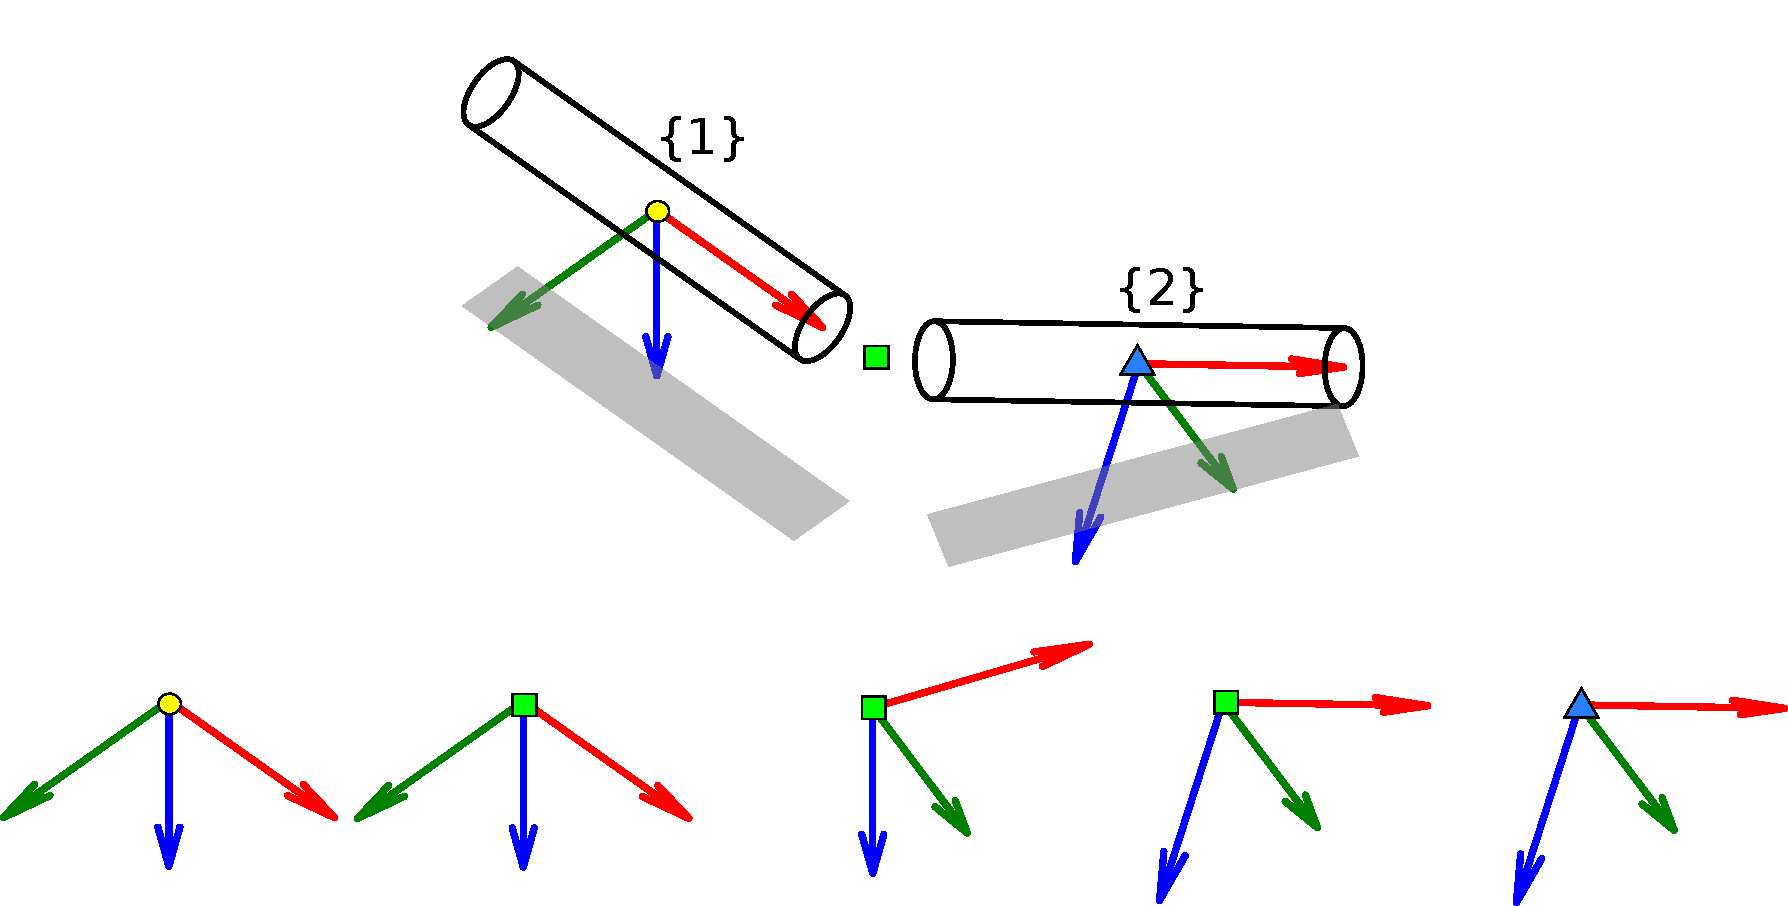
\includegraphics[width=\textwidth]{assets/transforms_all.pdf}
    \caption{Intermediate frames between frame $1$ and $2$.}
    \label{fig:transforms_all}
\end{figure}
It will be assumed that all the $\bm{B}_{i,j}(\theta)$ transformations can be written as
\begin{align}
    \bm{B}_{i,j}(0)\exp\left(\theta[\bm{b}_{i,j}]_{\wedge}\right),
\end{align}
where $\bm{b}_{i,j} \in \R^6$ is a constant vector. It it important to note that
this simple form can represent a lot of transformations in $\SE$. For instance,
a constant transform can be expressed by setting $\bm{b}_{i,j} = \bm{0}$ and choosing $\bm{B}_{i,j}(0)$.
Pure rotations of one variable can be parameterized using angle-axis parameters, using $\bm{b}_{i,j} =
\begin{bmatrix}\bm{0}^T & \bm{k}^T &\end{bmatrix}^T$, where $\bm{k}$ is the axis. Translations
are acheived by setting $\bm{b}_{i,j} = \begin{bmatrix} \bm{k}^T & \bm{0}^T \end{bmatrix}^T$.
More complex transforms, such as the one between frame $2$ and $1$ in \autoref{fig:transforms_all}
are acheived by consecutive transformations on this form. To illustrate this point, the transformation
from frame $2$ to frame $1$ in \autoref{fig:transforms_all} can be expressed as
\begin{align}
    \begin{bmatrix}1 & 0 & 0 & l_1 \\ 0 & 1 & 0 & 0 \\ 0 & 0 & 1 & 0 \\ 0 & 0 & 0 & 1\end{bmatrix}
    \exp\left(\theta_1\begin{bmatrix}\bm{0} \\ 0 \\ 0 \\ 1\end{bmatrix}_{\wedge}\right)
    \exp\left(\theta_2\begin{bmatrix}\bm{0} \\ 0 \\ 1 \\ 0\end{bmatrix}_{\wedge}\right)
    \begin{bmatrix}1 & 0 & 0 & l_2 \\ 0 & 1 & 0 & 0 \\ 0 & 0 & 1 & 0 \\ 0 & 0 & 0 & 1\end{bmatrix}.
\end{align}
Althoug the system has become much more general by allowing joint transformations to
be functions of an arbitrary number of parameters, computation of the link jacobians can
be done in a very similar way as previously shown. This is because the sequence of
transforms from frame $i+1$ to $i$ is parameterized in exactly the same way as
from $n$ to $1$ when the robot has joints of one parameter.

% ----------------
\iffalse
We define $\bm{\theta} = \begin{bmatrix}\theta_1 & \theta_2 & \cdots & \theta_{n-1}\end{bmatrix}^T$
and
\begin{align}
    \bm{A}_{i:j}(\bm{\theta}) =
    \begin{cases}
        \bm{A}_i(\theta_i) \bm{A}_{i+1}(\theta_{i+1}) \cdots \bm{A}_{j-1}(\theta_{j-1}) & i \leq j \\
        \bm{0}_{4 \times 4} & i > j \\
    \end{cases}.
\end{align}
It can be shown that the transformation matrix $\bm{A}_{i}(\theta_i)$ can be
expressed as \cite{murray2017}:
\begin{align}
    \bm{A}_i(\theta_i) &= \bm{A}_i(0) \exp([\bm{a}_i]_{\wedge} \theta_i), \label{eq:expmap}
\end{align}
for some $\bm{a}_i \in \R^6$. The body twist
of link $i+1$ relative to the inertial frame $n$ can be expressed as
\begin{subequations}
\begin{align}
    \bm{\nu}_{n(i+1)}^{i+1} &= \left(\bm{H}_{i+1}^n\right)^{-1} \dot{\bm{H}}_{i+1}^n \\
    &= \bm{A}_{1:i}^{-1}(\bm\theta) \bm{H}_1^{-1} \dot{\bm{H}}_{1} \bm{A}_{1:i}(\bm\theta) \nonumber \\
    &+ \bm{A}_{2:i}^{-1}(\bm\theta) [\bm{a}_1]_{\wedge}\bm{A}_{2:i}(\bm\theta) \dot{\theta}_1 \nonumber \\
    &\vdots \label{eq:body_twist_def} \\
    &+ \bm{A}_{i:i}^{-1}(\bm\theta) [\bm{a}_{i-1}]_{\wedge}\bm{A}_{i:i}(\bm\theta) \dot{\theta}_{i} \nonumber \\
    &+ [\bm{a}_{i}]_{\wedge} \dot{\theta}_i. \nonumber
\end{align}
\end{subequations}
Defining $\bm{\nu}_i := \bm{\nu}_{ni}^i$ as the body twist of link $i$ relative to
the inertial frame $n$, \autoref{eq:body_twist_def} can be written recursively as:
\begin{subequations}
    \label{eq:body_twist_recursive}
\begin{align}
    \bm{\nu}_{1} &= \bm{\nu}_{n1}^1 \\
    \bm{\nu}_{i+1} &= \Ad^{-1}(\bm{A}_i(\theta_i)) \bm{\nu}_i + [\bm{a}_i]_{\wedge} \dot{\theta}_i.
\end{align}
\end{subequations}
This motivates the definition of the link Jacobians that are defined in a way
such that
\begin{align}
    \bm{\nu}_{i} = \bm{J}_i(\bm{\theta}) \bm{\zeta}
\end{align}
where the body twist $\bm{\nu}$ and the joint velocities $\dot{\bm{\theta}}$ are
collected in the vector $\bm{\zeta}$:
\begin{align}
    \bm{\zeta} = \begin{bmatrix}\bm{\nu} \\ \dot{\bm{\theta}}\end{bmatrix} \in \R^{6+(n-1)}.
\end{align}
From \autoref{eq:body_twist_recursive} we can see that the link Jacobians can be
defined as
\begin{subequations}
    \label{eq:link_jacobian}
\begin{align}
    \bm{J}_1(\bm{\theta}) &= \begin{bmatrix} \bm{I}_6 & \bm{0}_{6 \times n} \end{bmatrix} \\
        \bm{J}_{i+1}(\bm{\theta}) &= \begin{bmatrix}
            \Ad^{-1}(\bm{A}_{1:i}(\bm{\theta}))  &  \Ad^{-1}(\bm{A}_{2:i}(\bm{\theta})) \bm{a}_1 &
            \cdots & \bm{a}_i & \bm{0}_{6 \times (n-i)}
        \end{bmatrix} \\
    &= \Ad^{-1}(\bm{A}_i(\theta_i)) \bm{J}_i(\bm{\theta}) + \begin{bmatrix}
        \bm{0}_{6 \times (5+i)} & \bm{a}_i & \bm{0}_{6 \times (n-i)}
    \end{bmatrix}.
\end{align}
\end{subequations}
The derivatives of the link Jacobians are needed for control purposes and
calculation of the Coriolis matrix. By differentiating \autoref{eq:link_jacobian}
with respect to time, we get
\begin{subequations}
\begin{align}
    \dot{\bm{J}}_1(\bm{\theta}) &= \bm{0}_{6\times(6+n)} \\
    \dot{\bm{J}}_{i+1}(\bm{\theta},\dot{\bm{\theta}}) &= -[\bm{a}_i]_{\wedge} \Ad^{-1}(\bm{A}_i(\theta_i))
        \bm{J}_i(\bm{\theta})\dot{\theta}_i + \Ad^{-1}(\bm{A}_i(\theta_i))\dot{\bm{J}}_i(\bm{\theta},\dot{\bm{\theta}}) \\
    &= -[\bm{a}_i]_{\wedge}\bm{J}_{i+1}(\bm{\theta})\dot{\theta}_i +
        \Ad^{-1}(\bm{A}_i(\theta_i))\dot{\bm{J}}_i(\bm{\theta},\dot{\bm{\theta}}).
\end{align}
\end{subequations}

\fi %--------------------------


\subsection{Dynamics}

For each link, $i$, defined in the previous subchapter, we associate the following
properties: $\bm{M}_i \in \R^{6 \times 6}$ is the inertia matrix of the link,
$\bm{J}_i \in \R^{6 \times (6+n)}$ is the link jacobian, $\bm{C}_i \in \R^{6 \times 6}$
is the Coriolis matrix, $\bm{D}_i \in \R^{6 \times 6}$ is the damping matrix and
$\bm{g}_i \in \R^{6}$ is the gravitational forces and hydrostatic forces and moments.
The damping matrix will be discussed in \autoref{sec:hydrodynamics}.
$\bm{M}_i$ takes into account the added mass of the link
\begin{align}
    \bm{M}_i &= \bm{M}_{RB,i} + \bm{M}_{A,i},
\end{align}
where $\bm{M}_{RB,i}$ is the rigid body inertia matrix of the link and $\bm{M}_{A,i}$
is the added mass matrix of the link. As a result of the added mass, the Coriolis
matrix is given by
\begin{align}
    \bm{C}_i &= \bm{C}_{RB,i} + \bm{C}_{A,i}
\end{align}
where $\bm{C}_{RB,i}$ is the Coriolis matrix of the rigid body and $\bm{C}_{A,i}$
is a function of the added mass matrix. The added mass matrix and the damping matrix
for each link is the topic of \autoref{sec:hydrodynamics}. The dynamics of the
system described in the previous subchapter can be modeled as
\cite{from2014}:
\begin{align}
    \bm{M}(\bm{\theta})\dot{\bm{\zeta}} +
        \bm{C}(\bm{\theta}, \bm{\zeta}) \bm{\zeta} +
        \bm{D}(\bm{\theta}, \bm{\zeta}) \bm{\zeta} +
        \bm{g}(\bm{\xi}) =
        \bm{\tau}. \label{eq:robot_dynamics}
\end{align}
$\bm{M}(\bm{\theta}) \in \R^{(6+n)\times(6+n)}$  is the inertia matrix of the
system, $\bm{C}(\bm{\theta}, \bm{\zeta}) \in \R^{(6+n)\times(6+n)}$ is the
Coriolis matrix, $\bm{D}(\bm{\theta}, \bm{\zeta}) \in \R^{(6+n)\times(6+n)}$ is
the damping matrix, $\bm{g}(\bm{\xi}) \in \R^{6+n}$ is the gravitational forces
and buoyancy forces and moments acting on the system, $\bm{\tau} \in \R^{n}$ is the generalized
forces acting on the system as a result of the actuators,
and $\bm{\tau}_{\mathrm{ext}} \in \R^{6+n}$ is the
generalized external forces acting on the system. Let $\bm{J}_{i}(\bm{\theta})$
be the link Jacobians as defined in \autoref{eq:link_jacobian}.
The inertia matrix
can be expressed as
\begin{align}
    \bm{M}(\bm{\theta}) &= \sum_{i=1}^{n} \bm{J}_{i}^T(\bm{\theta}) \bm{M}_i \bm{J}_{i}(\bm{\theta}).
\end{align}
Note that if the Jacobians are full rank, the inertia matrix is positive definite.
Furthermore, it is always symmetric. The Coriolis matrix can be expressed as
\begin{align}
    \bm{C}(\bm{\theta}, \bm{\zeta}) &=
    \sum_{i=1}^{n} \bm{J}_{i}^T(\bm{\theta}) \bm{M}_i \dot{\bm{J}}_{i}(\bm{\theta},\dot{\bm{\theta}})
    -\bm{J}_{i}^T(\bm{\theta}) \bm{C}_i(\bm{\theta},\bm{\zeta})_i \bm{J}_{i}(\bm{\theta}) \bm{\zeta}.
\end{align}
The damping matrix can be expressed as
\begin{align}
    \bm{D}(\bm{\theta}, \bm{\zeta}) &=
    \sum_{i=1}^{n} \bm{J}_{i}^T(\bm{\theta}) \bm{D}_i(\bm{\theta},\bm{\zeta}) \bm{J}_{i}(\bm{\theta}).
\end{align}
and the gravitational forces and buoyancy forces and moments can be expressed as
\begin{align}
    \bm{g}(\bm{\xi}) &=
    \sum_{i=1}^{n} \bm{J}_{i}^T(\bm{\theta}) \bm{g}_i(\bm{\xi}). \label{eq:modeling:g}
\end{align}
The control inputs $\bm{u}$ are mapped to the generalized forces $\bm{\tau}$ by
the actuator configuration matrix $\bm{B}(\bm{\theta})$ as
\begin{align}
    \bm{\tau} &= \bm{B}(\bm{\theta}) \bm{u} &
    \bm{B}(\bm{\theta}) &= \begin{bmatrix}
        \bm{J}_1^T(\bm{\theta}) \bm{B}_1 & \cdots & \bm{J}_n^T(\bm{\theta}) \bm{B}_n
    \end{bmatrix},
\end{align}
where $\bm{B}_i$ is the actuator configuration matrix for link $i$. For a simple
thruster configuration, such as in the case where all thrusters are fixed with
respect to some link, the $\bm{B}_i$ matrices are constant and can be expressed
as
\begin{align}
    \bm{B}_i &= \begin{bmatrix}
        \bm{\beta}_{t,i,1} & \cdots & \bm{\beta}_{t,i,m} \\
        \bm{r}_{t,i,1} \times \bm{\beta}_{t,i,1} & \cdots & \bm{r}_{t,i,m} \times \bm{\beta}_{t,i,m}
    \end{bmatrix},
\end{align}
where $\bm{\beta}_{t,i,j}$ is the direction of the thrust and $\bm{r}_{t,i,j}$
is the point of application of the thrust.





% -----------------------------------------------------------------------------
\section{Hydrodynamics}
\label{sec:hydrodynamics}

Hydrodynamics is the study of the forces acting on a body in a fluid. The forces
can be modeled as potential forces, giving rise to the added mass matrix, and
damping forces. This chapter will focus on how to model the hydrodynamic forces
acting on a rigid body in a fluid.

\subsection{Added Mass}

When a rigid body accelerates in a fluid, the fluid is accelerated as well. 
This contributes to the total kinetic energy of the system \cite{antonelli2018}.
To account for these effects, the spatial inertia matrix of the rigid body
can be augmented to approximate the total kinetic energy of the system: 
\begin{equation}
    \bm{M} = \bm{M}_{RB} + \bm{M}_{A}.
\end{equation}
The matrix $\bm{M}_A$ is in reality a function of the wave excitation frequency
of the waves in the ocean \cite{fossen2021}. Because of the complex computations
of $\bm{M}_A(\omega)$, as well as the fact that for large vessels the natural
frequencies of the vessel are much lower than the wave excitation frequencies,
the added mass matrix is approximated as the zero-frequency added mass matrix
\begin{align}
    \bm{M}_A(\omega) &\approx \bm{M}_A(0)
\end{align}
Under this assumption, the kinetic energy of the fluid $T_A$ is approximated
as
\begin{align}
    T_a &= \frac{1}{2}\bm{\nu}^T\bm{M}_A\bm{\nu} & \dot{\bm{M}}_A &= \bm{0},
\end{align}
where $\bm{\nu}$ is the twist velocity of the rigid body. For underwater 
vehicles at low speed where the the shape has three planes of symmetry, the
added mass matrix can be approximated as \cite{fossen2021}:
\begin{align}
    \bm{M}_A = \bm{M}_A^T =
    -\operatorname{diag}(X_{\dot{u}}, Y_{\dot{v}}, Z_{\dot{w}},
        K_{\dot{p}}, M_{\dot{q}}, N_{\dot{r}}).
\end{align}
According to \cite{fossen2021} this approximation is found to be quite good for
many applications due to the fact that the off diagonal coupling terms are small
compared to the diagonal terms.

By applying strip theory the added mass matrix for a cylindrical rigid body of
mass $m$, length along the x-axis $l$ and radius $r$ can be derived as \cite{fossen1994}:
\begin{align}
 X_{\dot{u}} &= -0.1 m &
 Y_{\dot{v}} &= -\pi \rho r^2 l \nonumber \\
 Z_{\dot{w}} &= -\pi \rho r^2 l &
 K_{\dot{p}} &= 0 \\
 M_{\dot{q}} &= -\frac{1}{12} \pi \rho r^2 l^3 &
 N_{\dot{r}} &= -\frac{1}{12} \pi \rho r^2 l^3 \nonumber
\end{align}
where $\rho$ is the density of the fluid. For a three-dimensional ellipsoid with
lengths $a$, $b$ and $c$ along the x, y and z axis respectively, the added mass
can be approximated as \cite{fossen2021}:
\begin{align}
 X_{\dot{u}} &= -\frac{\alpha_0}{2-\alpha_0}m &
 Y_{\dot{v}} &= -\frac{\beta_0}{2-\beta_0}m \nonumber \\
 Z_{\dot{w}} &= Y_{\dot{v}}&
 K_{\dot{p}} &= 0 \label{eq:ellipsoid_added_mass} \\
 M_{\dot{q}} &= -\frac{1}{5}\frac{(b^2-a^2)^2(\alpha_0-\beta_0)}{2(b^2-a^2) + (b^2+a^2)(\beta_0-\alpha_0)}m&
 N_{\dot{r}} &= M_{\dot{q}} \nonumber
\end{align}

\subsection{Damping}

There are several phenomena that contribute to the damping of a rigid body in
a fluid. Among these are potential damping, skin friction, wave drift damping,
damping due to vortex shedding and lifting forces. In many cases
all of these effects can be approximated using a linear damping matrix $\bm{D}$ and
a quadratic damping matrix $\bm{D}_n$ \cite{fossen2021}. Damping can be modeled
as
\begin{align}
    \bm{D}(\bm{\nu}_r) &= \bm{D} + \bm{D}_n(\bm{\nu}_r) \\
    \bm{\tau}_d &= \bm{D}(\bm{\nu}_r)\bm{\nu}_r
\end{align}
for a 6-DOF rigid body, $\bm{D}(\bm{\nu}_r)$ is a $6\times 6$ matrix, $\bm{\nu}_r$
is the twist of the rigid body relative to the fluid and $\bm{\tau}_d \in \R^6$
is a vector of the damping forces and moments acting on the rigid body. \cite{antonelli2018}
states that the damping matrix can be approximated as
\begin{subequations}
\begin{align}
    \bm{D} &= -diag(X_u, Y_v, Z_w, K_p, M_q, N_r) \\
    \bm{D}_n &= -diag(X_{u|u|}|u|, Y_{v|v|}|v|, Z_{w|w|}|w|, K_{p|p|}|p|, M_{q|q|}|q|, N_{r|r|}|r|),
\end{align}
\end{subequations}

for completely submerged bodies. This will neglect coupling and dissipative effects.
It has been shown that by using strip theory, the damping force and
moment on a cylinder can be approximated by the follwing integrals \cite{mcmillan1995}:
\begin{subequations}
    \label{eq:cylinder_damping}
    \begin{align}
        \bm{f}_d &= - \rho C_D r \int_{0}^{l} ||\bm{v}^n(x)|| \bm{v}^n(x) \,dx \\
        \bm{m}_d &= - \rho C_D r \int_{0}^{l} ||\bm{v}^n(x)||
        \left(\begin{bmatrix}x & 0 & 0\end{bmatrix}^T \times \bm{v}^n(x)\right) \,dx,
    \end{align}
\end{subequations}
where $r$ and $l$ are the radius and length of the cylinder, $\rho$ the density
of the fluid, $C_D$ the drag coefficient and $\bm{v}^n(x)$ the velocity of the
fluid at the point $x$ along the length of the cylinder. Using the results stated
in \autoref{eq:cylinder_damping}, \citeauthor{schmidt2018} proposes a linear
damping matrix for a cylinder as \cite{schmidt2018}:
\begin{align}
    \bm{D} = \rho \pi l C_D v_{ref}
    \begin{bmatrix}
        \beta &            0 &             0 &          0 &              0 &            0 \\
            0 &            1 &             0 &          0 &              0 & \frac{1}{2}l \\
            0 &            0 &             1 &          0 &  -\frac{1}{2}l &            0 \\
            0 &            0 &             0 & \gamma r^2 &              0 &            0 \\
            0 &            0 & -\frac{1}{2}l &          0 & \frac{1}{3}l^2 &            0 \\
            0 & \frac{1}{2}l &             0 &          0 &              0 & \frac{1}{3}l^2
    \end{bmatrix},
\label{eq:damping_cyl}
\end{align}
where $C_D$, $v_{ref}$, $\beta$, $\gamma$ are constants to be determined.

% -----------------------------------------------------------------------------
\iffalse
\section{UVMS Kinematics}

The following chapter will descibe the kinematics of an \gls{uvms}
The \gls{uvms} consists of a rigid base and is connected to
a manipulator with $n$ links. This makes the \gls{uvms} have a snake-like structure.
Adopting notation from \cite{fossen2021}, the rigid base can be uniquely described
by a set of $6$ coordinates
\begin{align}
    \bm{\eta} &= \begin{bmatrix} \bm{p} \\ \bm{\Theta} \end{bmatrix} \in \R^6 &
        \bm{p} &= \begin{bmatrix} x^n \\ y^n \\ z^n \end{bmatrix} \in \R^3 &
    \bm{\Theta} &= \begin{bmatrix} \phi \\ \theta \\ \psi \end{bmatrix} \in \R^3,
\end{align}
where $\bm{p}$ is the position of the base described in a NED frame and $\bm{\Theta}$
are the Euler angles describing the orientation of the base. Note that the Euler
angles are singular at $\theta = \pm \pi/2$, and that using quaternions
would avoid this problem. Introducing quaternions would however add an extra
equality constraint to the system, making the system harder to simulate. Because
of this, Euler angles are used in this thesis. 

We assume the position of the manipulator links relative to the base are uniquely
described by a set of $n$


% -----------------------------------------------------------------------------
\section{UMS Dynamics}



% mention that the damping matrix is a function of the velocity of the body
% mention that for UVMs the damping matrix can be assumed decoupled for all links.

{
    \color{red}
    \begin{itemize}
        \item Multi-body dynamics
        \item Hydrodynamics (damping)
        \item Jacobians
        \item Inspiration from Henrik?
    \end{itemize}
}
\fi
